%%
%% res_trapping_probabilities.tex
%% 
%% Made by Robert Patro
%% Login   <rob@gvilwks03>
%% 
%% Started on  Tue Mar  9 13:18:45 2010 Robert Patro
%% Last update Tue Mar  9 13:18:45 2010 Robert Patro
%%

We evaluate the trapping probability for particles under the effect of
both a stationary and moving laser.  The trapping probabilities are
estimated on a discrete grid of positions relative to the focus of the
laser.  In all of our experiments, we consider a grid whose extents
match that of the discrete laser force grid $F$.  We sample this
grid in the $y$ and $z$ directions at a resolution of
$\SI{0.25}{\micro\meter}$.

\subsubsection{Trapping Probabilities under a Stationary Laser}

%Figures~\ref{fig:trapping-prob-static-gpu}
%and~\ref{fig:trapping-prob-static-cpu} illustrate how the probability
%of trapping a particle varies with respect to the particle's distance
%from the laser in both the $y$ and $z$ directions, under the influence
%of a stationary laser.  To verify the accuracy of our trapping
%probability estimates, we examine how the estimates computed using our
%GPU implementation differ from those computed using a CPU-based
%implementation of the same particle dynamics model.  Since the
%underlying governing equations are the same, and we perform a
%sufficient number of simulations (i.e. $1024$ per grid position) to
%ensure $95\%$ confidence in our probability estimate, we expect to see
%very little different between the two plots.  Indeed, an examination
%of Figures ~\ref{fig:trapping-prob-static-gpu}
%and~\ref{fig:trapping-prob-static-cpu} satisfies this expectation.

%We compute how the probability
%of trapping a particle varies with respect to the particle's distance
%from the laser in both the $y$ and $z$ directions, under the influence
%of a stationary laser. 
Figures~\ref{fig:trapping-prob-static-gpu} illustrates how the probability
of trapping a particle varies with respect to the particle's distance
from the laser in both the $y$ and $z$ directions, under the influence
of a stationary laser. To verify the accuracy of our trapping
probability estimates, we examine how the estimates computed using our
GPU implementation differ from those computed using a CPU-based
implementation of the same particle dynamics model. Since the
underlying governing equations are the same, and we perform a
sufficient number of simulations (i.e. $1024$ per grid position) to
ensure $95\%$ confidence in our probability estimate, we expect to see
very little difference between the two plots. Figure~\ref{fig:trapping-prob-static-cpu-gpu-error} 
shows the difference in probability estimates between the two implementations.
The average error between the CPU and the GPU implementation of the
probability estimate (computed using L2 norm) is $0.00091$.


\begin{figure}[htb!]
%%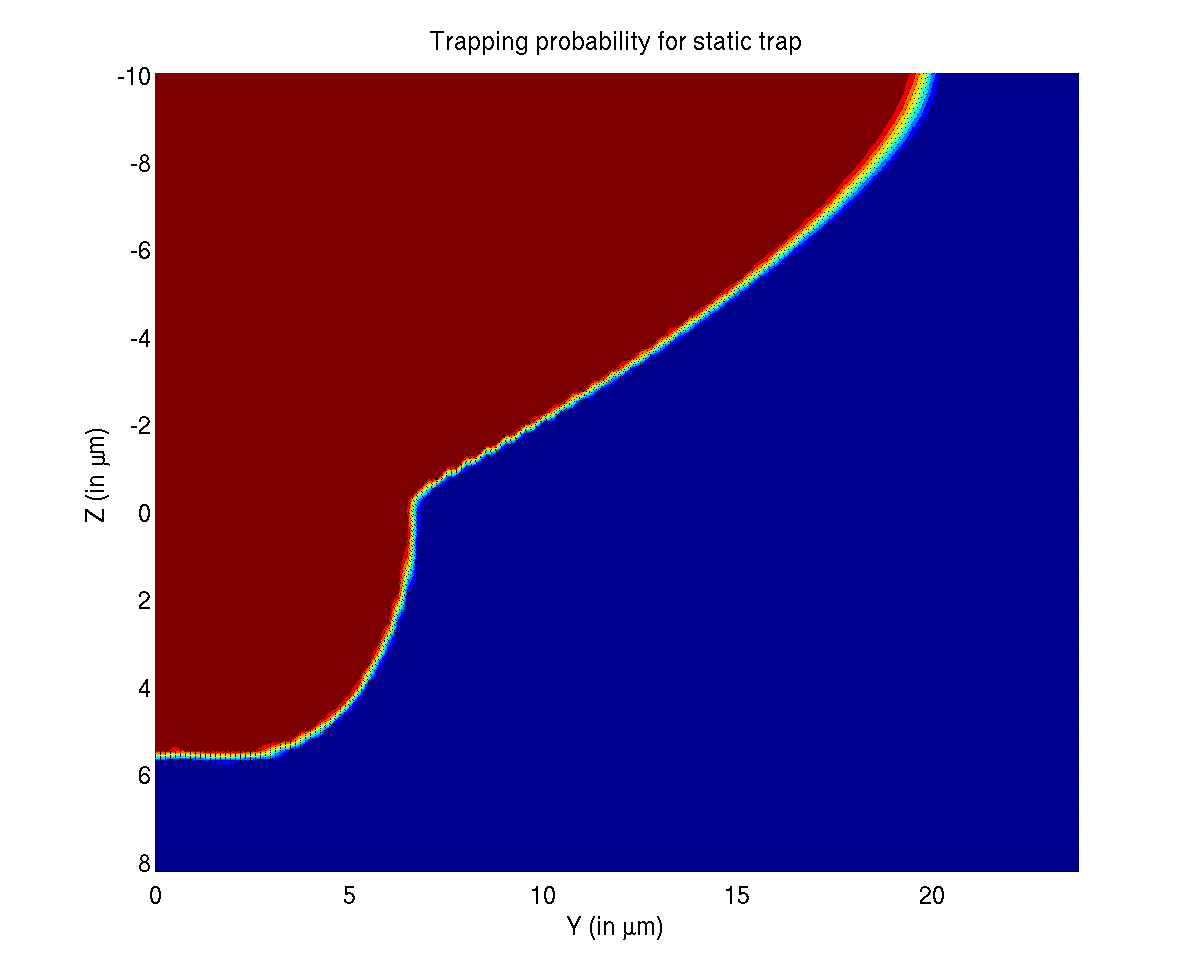
\includegraphics[width=\columnwidth]{figures/gpu_static_trap_prob_1_0s}
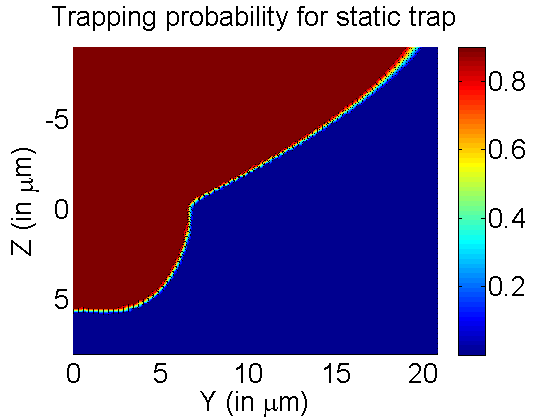
\includegraphics[width=\columnwidth]{figures/gpu_static_trap_prob_1024_particles}
\caption{This plot shows the probability of trapping a particle under
  the force exerted by a stationary laser with its focus at $(0,0)$,
  and was generated using the GPU implementation detailed in this paper.}
\label{fig:trapping-prob-static-gpu}
\end{figure}

%\begin{figure}[htb!]
%%%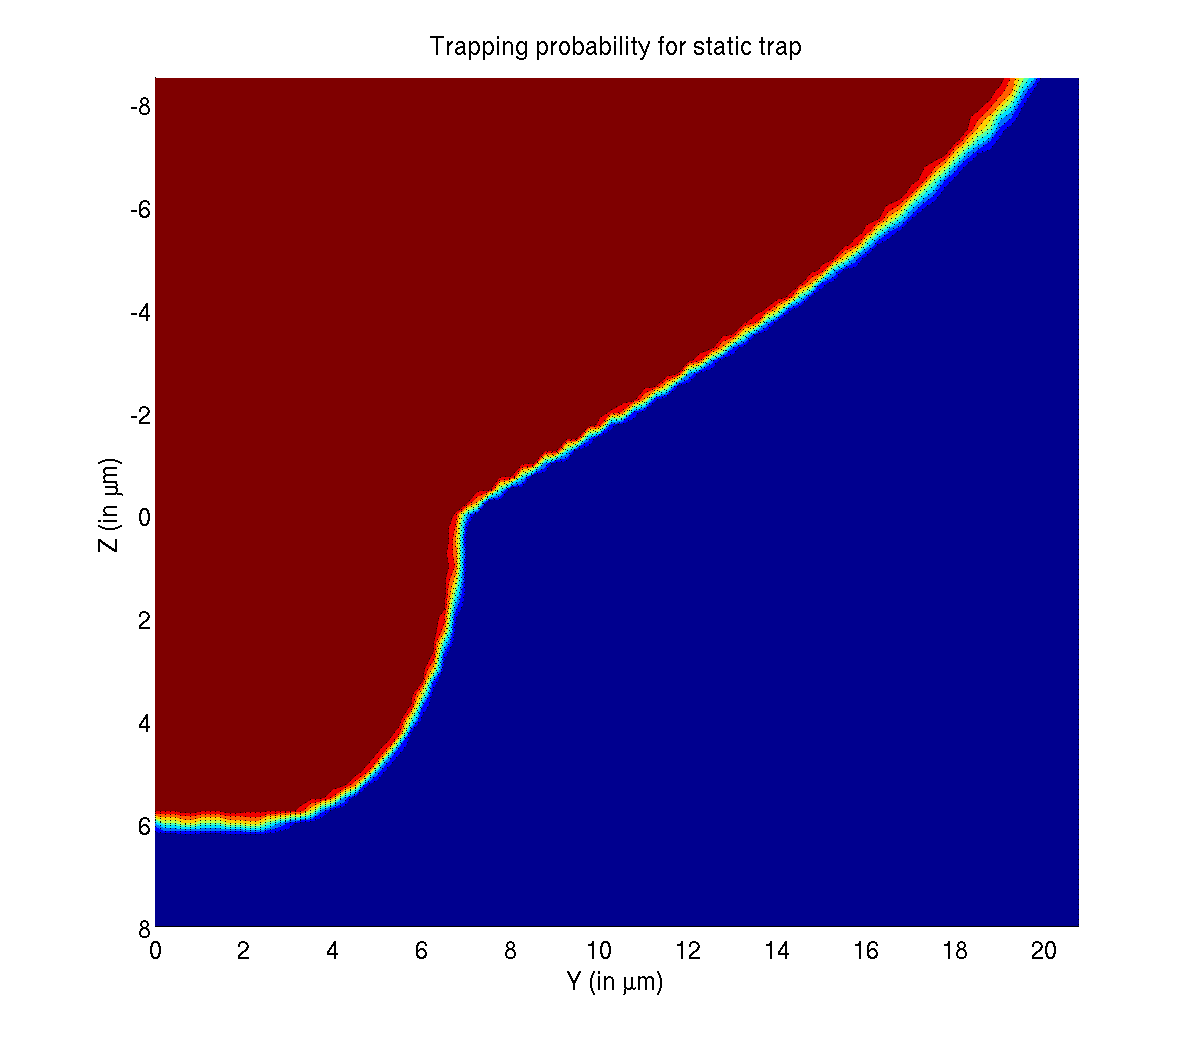
\includegraphics[width=\columnwidth]{figures/cpu_static_trap_prob_1_0s}
%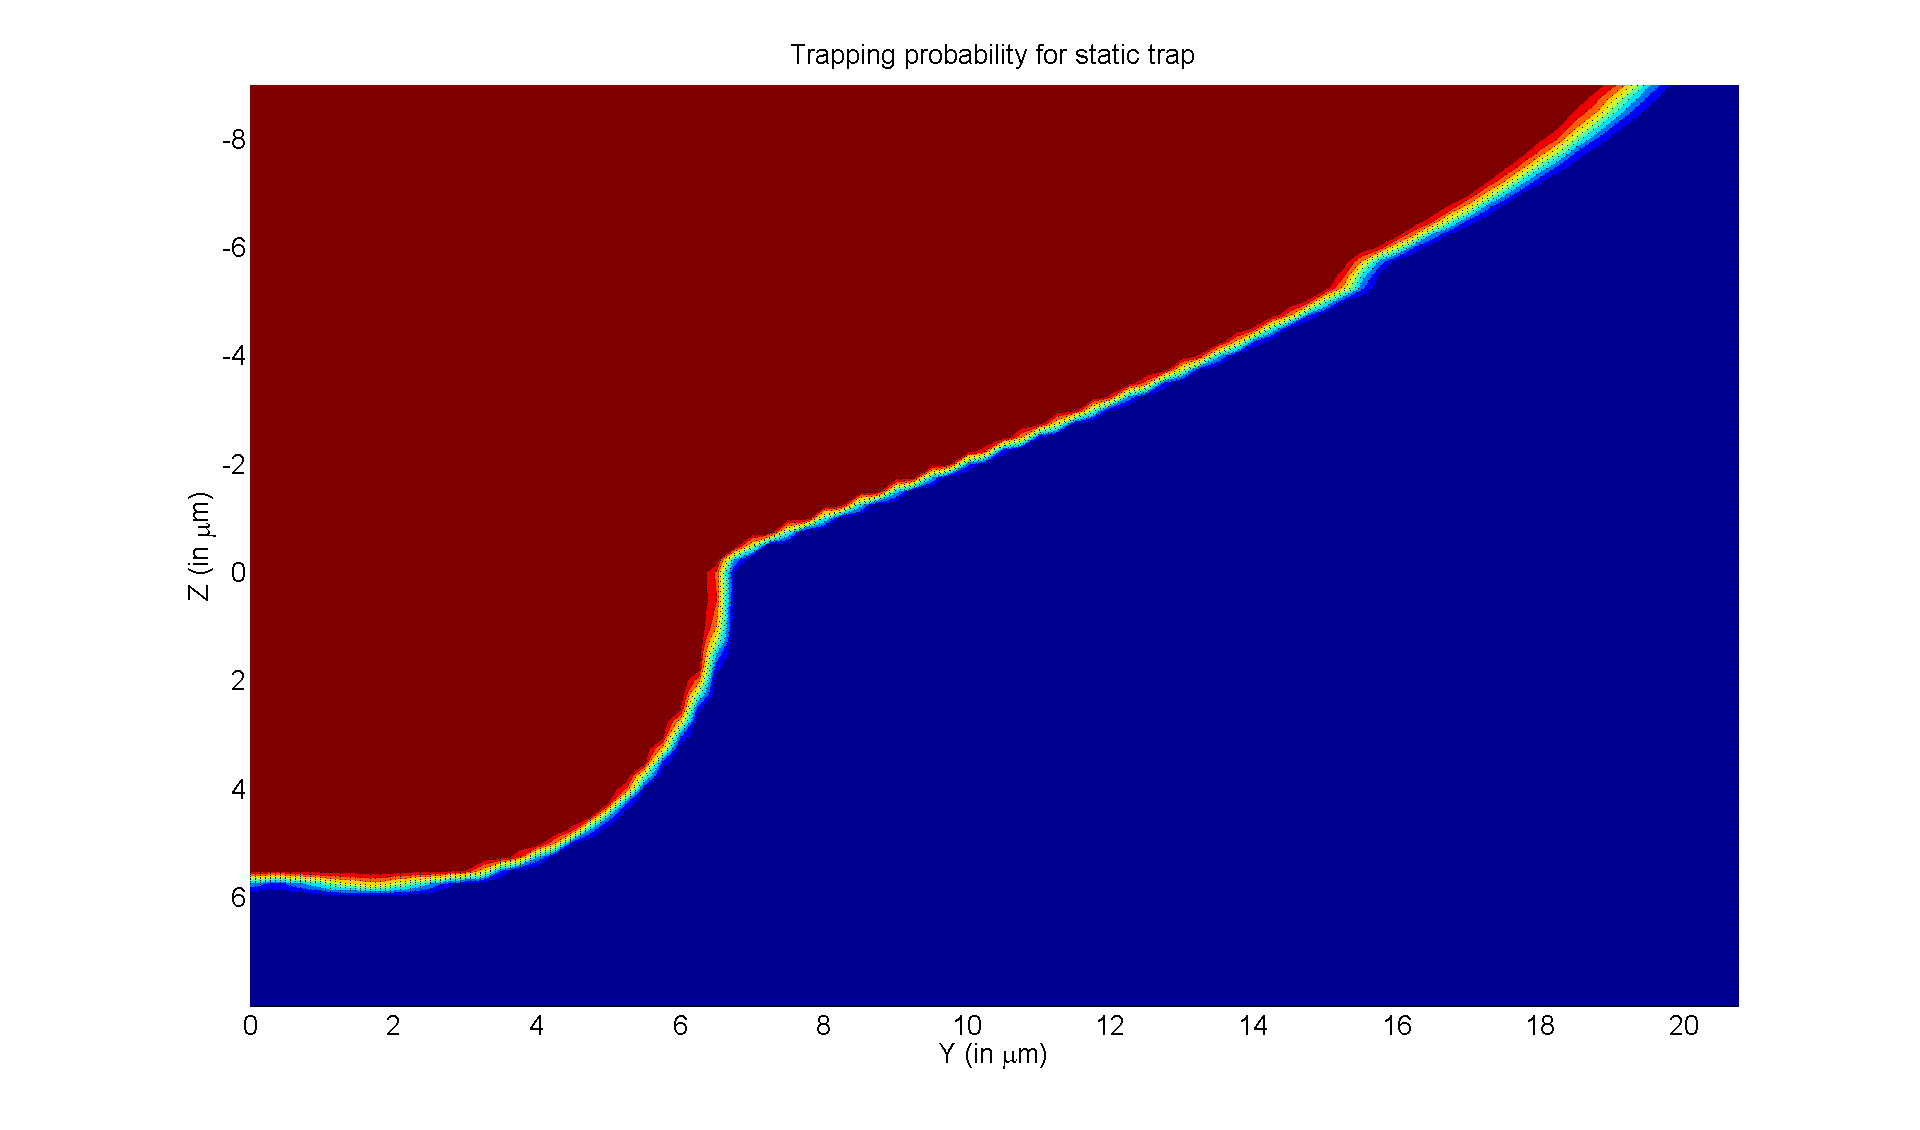
\includegraphics[width=\columnwidth]{figures/cpu_static_trap_prob_1024_particles}
%\caption{This plot shows the probability of trapping a particle under
%  the force exerted by a stationary laser with its focus at $(0,0)$.
%  This plot was generated using a CPU based implementation.}
%\label{fig:trapping-prob-static-cpu}
%\end{figure}

\begin{figure}[htb!]
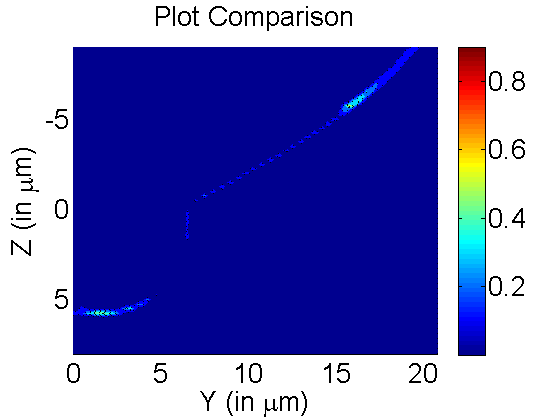
\includegraphics[width=\columnwidth]{figures/absolute_error}
\caption{
This plot shows the absolute difference between the CPU and the 
GPU implementation of the probability of trapping a particle under 
the force exerted by a stationary laser with its focus at $(0,0)$.
}
\label{fig:trapping-prob-static-cpu-gpu-error}
\end{figure}


We also examine the difference between probability estimates computed 
using single and double precision. We found the average error 
(computed using L2 norm) to be $ 0.00084$.


%\begin{figure}[htb!]
%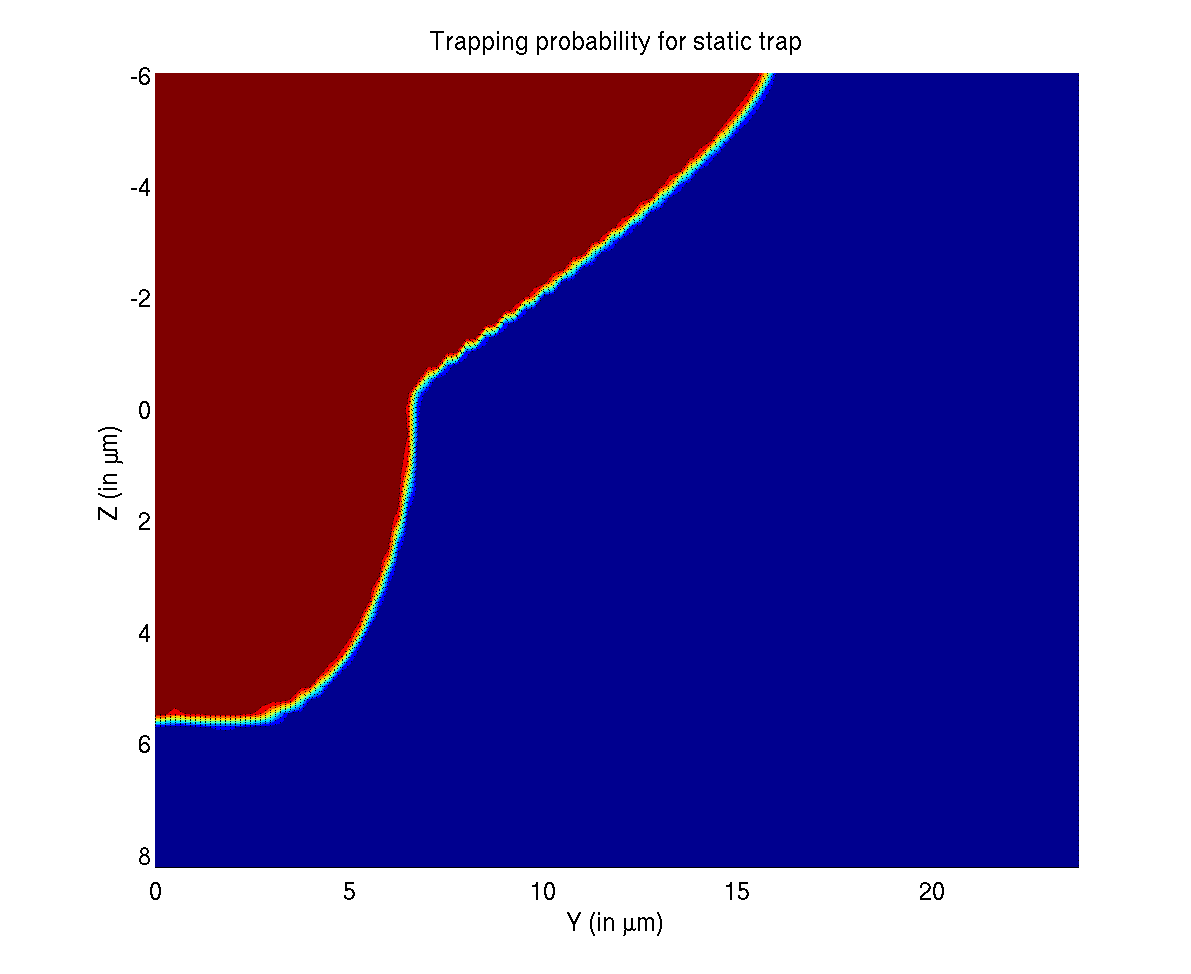
\includegraphics[width=\columnwidth]{figures/gpu_static_trap_prob_0_5s}
%\caption{This plot shows the probability of trapping a particle under
%  the force exerted by a stationary laser with its focus at $(0,0)$,
%  and was generated using the GPU implementation detailed in this
%  paper; the simulation duration was $0.5$s.}
%\label{fig:trapping-prob-static-gpu-0-5}
%\end{figure}
%
%
%\begin{figure}[htb!]
%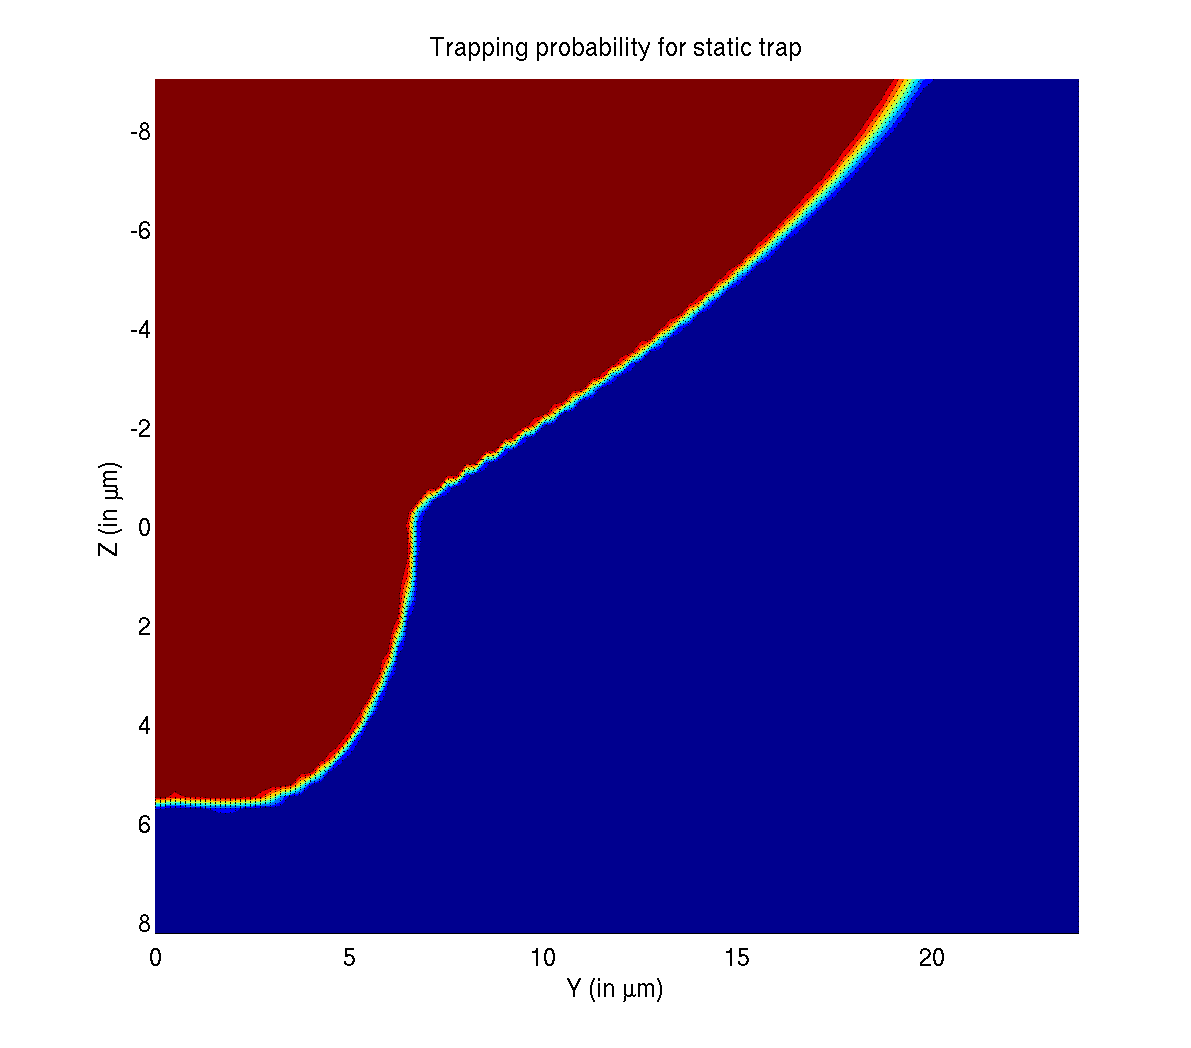
\includegraphics[width=\columnwidth]{figures/gpu_static_trap_prob_1_5s}
%\caption{This plot shows the probability of trapping a particle under
%  the force exerted by a stationary laser with its focus at $(0,0)$,
%  and was generated using the GPU implementation detailed in this
%  paper; the simulation duration was $1.5$s.}
%\label{fig:trapping-prob-static-gpu-1-5}
%\end{figure}
%
%\begin{figure}[htb!]
%%%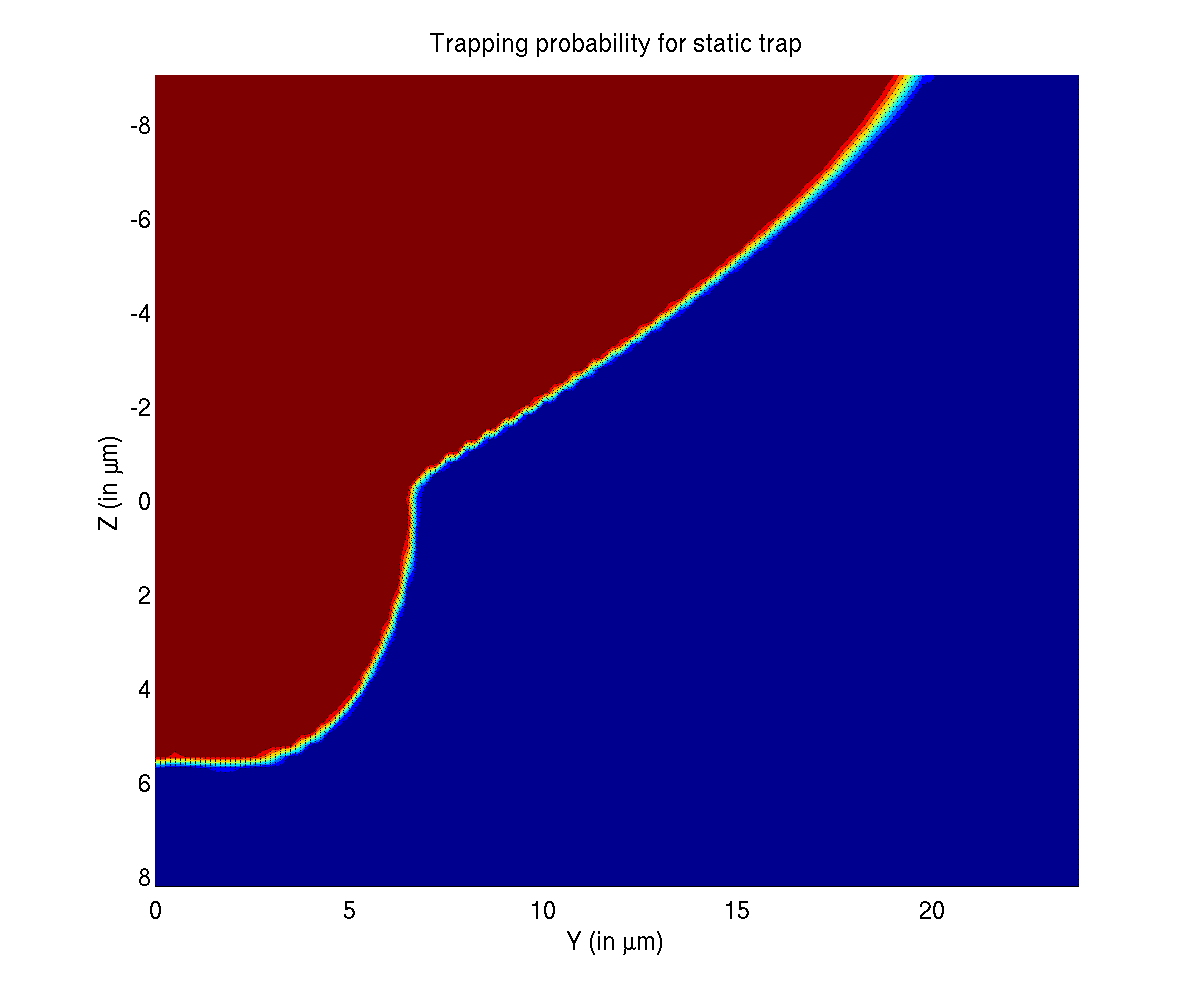
\includegraphics[width=\columnwidth]{figures/gpu_static_trap_prob_2_0s}
%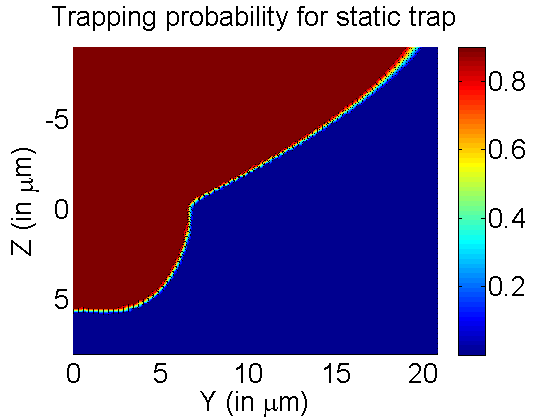
\includegraphics[width=\columnwidth]{figures/gpu_static_trap_prob_1024_particles}
%\caption{This plot shows the probability of trapping a particle under
%  the force exerted by a stationary laser with its focus at $(0,0)$,
%  and was generated using the GPU implementation detailed in this
%  paper; the simulation duration was $2.0$s.}
%\label{fig:trapping-prob-static-gpu-2-0}
%\end{figure}

\subsubsection{Trapping Probabilities under a Moving Laser}

Figures~\ref{fig:trapping-prob-xyvel-gpu}, and \ref{fig:trapping-prob-zvel-gpu}
%\ref{fig:trapping-prob-xyvel-cpu}, , and
%\ref{fig:trapping-prob-zvel-cpu} 
illustrate how the probability of
trapping a particle varies with respect to the particle's distance from
the laser in both the $y$ and $z$ directions, under the influence of a
moving laser.  In particular, we consider a laser moving with a
constant velocity of $\SI{0.65}{\micro\meter\per\milli\second}$
in the $y$ direction as well as a laser moving with a constant
velocity of $\SI{0.325}{\micro\meter\per\milli\second}$ in the
$z$ direction.

\begin{figure}[htb!]
  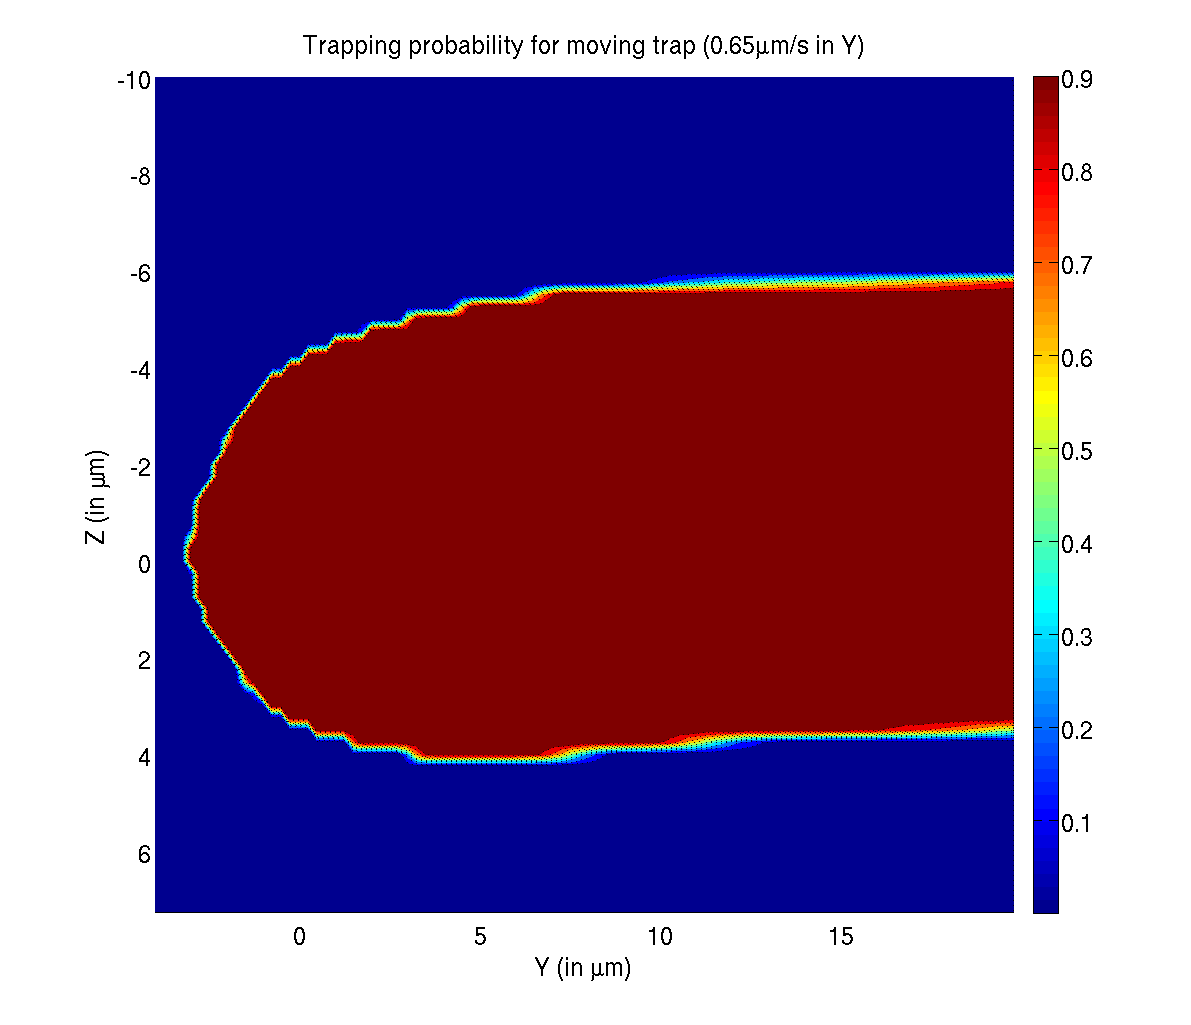
\includegraphics[width=\columnwidth]{figures/gpu_moving_0_65_y}
\caption{
  This plot shows the probability of trapping a particle under
  the force exerted by laser moving at a constant velocity of
  $\SI{0.65}{\micro\meter\per\milli\second}$ in the direction
  $(1,0)$, and was generated using the GPU implementation detailed in 
  this paper.
}

\label{fig:trapping-prob-xyvel-gpu}
\end{figure}


% \begin{figure}[htb!]
% \caption{
%   This plot shows the probability of trapping a particle under
%   the force exerted by laser moving at a constant velocity of
%   $\SI{0.65}{\frac{\micro\meter}{\milli\second}}$ in the direction
%   $(1,0)$, and was generated using a CPU-based implementation.
% }
% \label{fig:trapping-prob-xyvel-cpu}
% \end{figure}

\begin{figure}[htb!]
  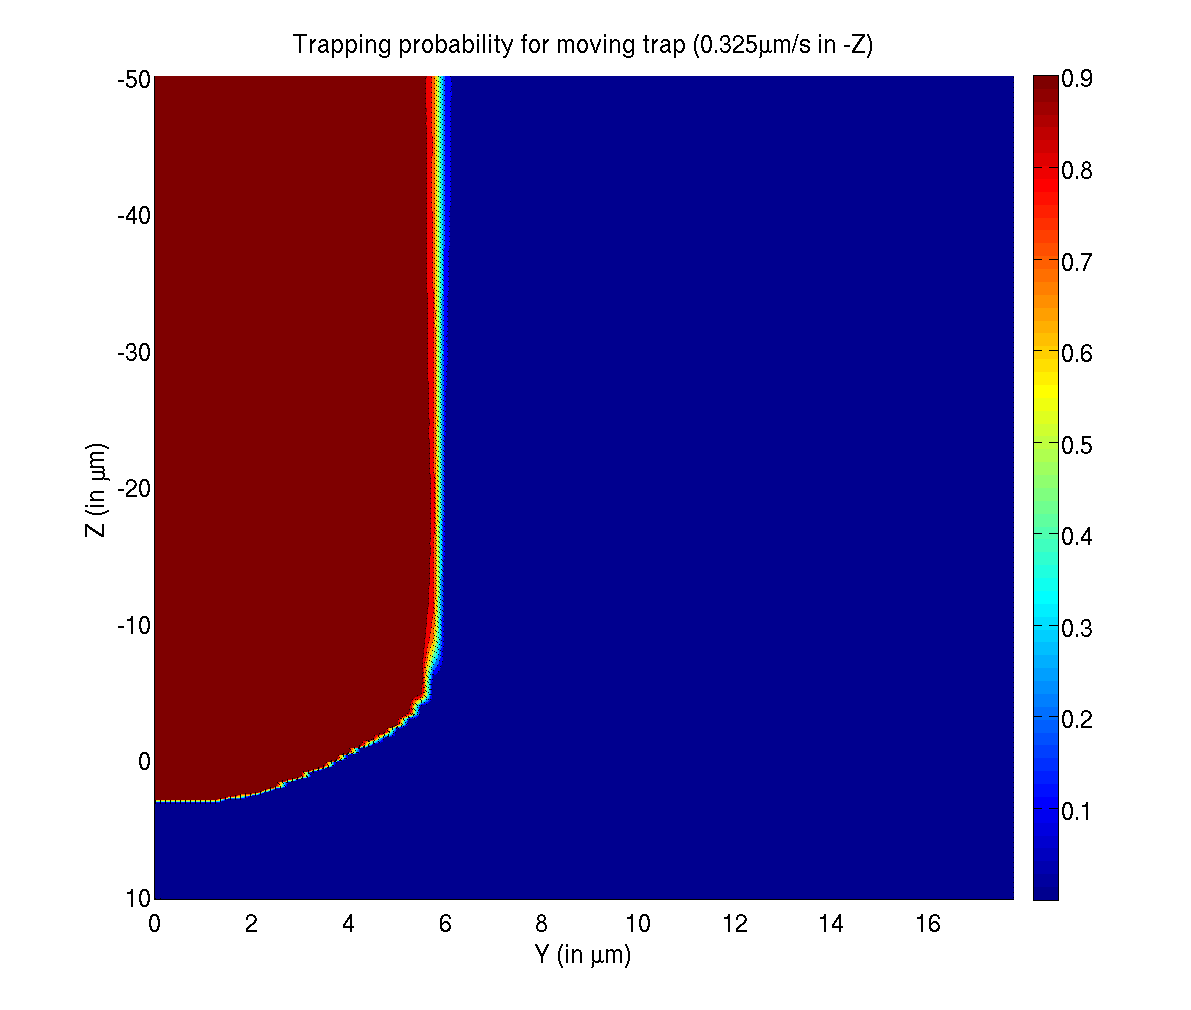
\includegraphics[width=\columnwidth]{figures/gpu_moving_0_325_z}
\caption{
  This plot shows the probability of trapping a particle under
  the force exerted by laser moving at a constant velocity of
  $\SI{0.325}{\micro\meter\per\milli\second}$ in the direction
  $(0,-1)$, and was generated using the GPU implementation detailed in 
  this paper.
}
\label{fig:trapping-prob-zvel-gpu}
\end{figure}

% \begin{figure}[htb!]

% \caption{
%   This plot shows the probability of trapping a particle under
%   the force exerted by laser moving at a constant velocity of
%   $\SI{0.325}{\frac{\micro\meter}{\milli\second}}$ in the direction
%   $(0,-1)$, and was generated using a CPU-based implementation.
% }
% \label{fig:trapping-prob-zvel-cpu}
% \end{figure}



%%% Local Variables: 
%%% mode: latex
%%% TeX-master: t
%%% End: 
